\documentclass[a4paper,11pt]{article}
\usepackage{geometry}
 \geometry{
 a4paper,
 total={170mm,257mm},
 left=20mm,
 top=20mm,
 }


 \usepackage{multirow}
\usepackage{colortbl}
 \usepackage{hhline}
 \usepackage{lipsum}  %%% Lorem ipsum

\setlength{\headheight}{30.0pt}
\setlength{\footskip}{20pt}

  \usepackage{colortbl}
\usepackage{booktabs}

\usepackage{hyperref}
\hypersetup{
    colorlinks=True,
    linkcolor={blue!20!black},
    filecolor=magenta,      
    urlcolor=cyan,
}



 \usepackage[export]{adjustbox}
\usepackage[english]{babel}
\usepackage[utf8]{inputenc}
\usepackage{fancyhdr}
\usepackage{multicol}

\pagestyle{fancy}
\fancyhf{}
\rhead{\textit{Pul074BEX004}}
\lhead{\textit{Amrit Prasad Phuyal}}
\rfoot{\thepage}


\usepackage{mathpazo} % Palatino font
\usepackage{graphicx}
\usepackage{float}


%%%% Anser environment use %%%% Anser environment use %%%% Anser environment use \input{./AnsENV.tex}
%% use \begin{A... {**** argument***}
\RequirePackage{scrextend}

\newenvironment{A}[1]{\textit{Answer:}{\begin{addmargin}[2em]{2em}{#1}\end{addmargin} 
  }}

% just leave some space   
%% use \begin{A... {**** argument***}
\RequirePackage{scrextend}

\newenvironment{A}[1]{\textit{Answer:}{\begin{addmargin}[2em]{2em}{#1}\end{addmargin} 
  }}

% just leave some space   
%% use \begin{A... {**** argument***}
\RequirePackage{scrextend}

\newenvironment{A}[1]{\textit{Answer:}{\begin{addmargin}[2em]{2em}{#1}\end{addmargin} 
  }}

% just leave some space    %% Answer environment 

%%% Question Environment%%%  use 
%%% Question Environment%%%  use 
%%% Question Environment%%%  use \input{./QueENV.tex}   to include
%% Use \begin{Q}....\end{Q}

\newcounter{QC}
\setcounter{QC}{1}
\newenvironment{Q}[1]{
    \section{Question -\arabic{QC}} \stepcounter{QC}{\large\textbf{#1}}
}

%%% Question Environment%%%

   to include
%% Use \begin{Q}....\end{Q}

\newcounter{QC}
\setcounter{QC}{1}
\newenvironment{Q}[1]{
    \section{Question -\arabic{QC}} \stepcounter{QC}{\large\textbf{#1}}
}

%%% Question Environment%%%

   to include
%% Use \begin{Q}....\end{Q}

\newcounter{QC}
\setcounter{QC}{1}
\newenvironment{Q}[1]{
    \section{Question -\arabic{QC}} \stepcounter{QC}{\large\textbf{#1}}
}

%%% Question Environment%%%

 %% Question Environment 
%%%%%% include  Titles.%%%% use \input{./CP}%%%
%%%use """"""""    \CP{}{}{}{}   """" %%%% and 4 argument to craete Title page 
%%%%%%%%%%%%%%%%%%%%%%%%%%%%%%%%%%%%%%%%%%%%%%%%%%%%%%%%%%%%%%%%%
%%%argument number
%% 1=major header ## Course name 
%% 2=minor4 heading ## lab/assignmet no
%% 3=Title  ## Assignment or Lab title
%% 4=submitted to::## input receiver Name"
%%%%%%%%%%%%%%%%%%%%%%%%%%%%%%%%%%%%%%%%%%%%%%%%%%%%%%%%%%%%%%%%%


\usepackage{mathpazo} % Palatino font
\usepackage{graphicx}
\usepackage{float}

%%% format and command for lab ans c and assembly

\newcommand{\HRule}{\rule{\linewidth}{0.4mm}} % Defines a new command for horizontal lines, change thickness here



%----------------------------------------------------------------------------------------
%	TITLE PAGE
%----------------------------------------------------------------------------------------


\newcommand{\CP}[4]{ \begin{titlepage} % Suppresses displaying the page number on the title page and the subsequent page counts as page 1
		%%%%  univerdity logo%%
		\begin{figure}[H]
			\centering
			
\includegraphics[scale=0.13]{tulogo.jpg}
		\end{figure}
		%%% end university logo

		\center % Centre everything on the page

		%------------------------------------------------
		%	Headings
		%------------------------------------------------

		\textsc{\huge Institute of Engineering \\ Central Campus,Pulchowk}\\[1.5cm] % Main heading such as the name of your university/college

		\textsc{\Large #1}\\[0.5cm] % Major heading such as course name

		\textsc{\large #2}\\[0.5cm] % Minor heading such as assignment no./ lab no.

		%------------------------------------------------
		%	Title
		%------------------------------------------------

		\HRule\\[0.4cm]

		{\Huge\bfseries #3}\\[0.4cm] % Title of your document

		\HRule\\[1.5cm]

		%------------------------------------------------
		%	Author(s)
		%------------------------------------------------
		\vfill\vfill
		\begin{minipage}{0.4\textwidth}
			\begin{flushleft}
				\large{
				\textbf{Submitted BY:}\\
				{\normalsize AMRIT PRASAD PHUYAL}\\ % NAME
				{\normalsize Roll: PULL074BEX004}} % Roll
			\end{flushleft}
		\end{minipage}
		~
		\begin{minipage}{0.4\textwidth}
			\begin{flushright}
				\large
				\textbf{Submitted To:}\\
				{ \normalsize{#4}\\ }% recepent's  Name 
				{\normalsize Department of Electronics and Computer Engineering}
			\end{flushright}
		\end{minipage}

		%------------------------------------------------
		%	Date
		%------------------------------------------------

		\vfill\vfill\vfill % Position the date 3/4 down the remaining page

		{\large\today} % Date, change the \today to a set date if you want to be precise

		\vfill % Push the date up 1/4 of the remaining page

	\end{titlepage}
} %%% cover page
 %%%%%% generate table from https://truben.no/table/ and paste bwtween \begin{DT} and end
%% use \input{./diffTable.tex}

\usepackage[table]{xcolor}
\usepackage{array}
\rowcolors{2}{blue!20}{white}
\newcommand{\head}[1]{%
   \textcolor{black}{\textbf{#1}}}
   
\renewcommand{\arraystretch}{1.5}

\setlength{\arrayrulewidth}{0.5mm}
\newenvironment{DT}[2]
{\begin{table}[H]
   \centering
   \sffamily
   \newcommand{\Cap}{\caption{#1 VS #2}}
 \begin{tabular}{|>{\cellcolor{cyan!15}\color{black!100}\bfseries}m{3.5cm}| m{6.5cm}| m{6.5cm}|}
     \rowcolor{cyan!15}
     \hline
     \head{KEYS} & \head{#1} & \head{#2} \\ \hline \hline
    } 
    {
    \hline
  \end{tabular}
  \Cap
\end{table}
} %% Diff table environment 


\begin{document}


%%%%  COver page 
\CP{Computer Network}{Assignmnent \#3}{Computer Network Assignmnent \#3}
{SHARAD KUMAR GHIMIRE}
%%%%%%%%%%%%%%%%%%%%

\pagenumbering{gobble}
\renewcommand{\contentsname}{Table of Contents}
\tableofcontents

%\pagebreak
%\listoffigures
\pagebreak
\listoftables

\pagebreak
\listoffigures
\pagebreak
\pagenumbering{arabic}

%%%%%%%%%%%%%%%%%%%%%%%%%%%%%%%%%%%11111111111111111111111111111111


\begin{Q}
    {
        List out typical features of the following networking devices:
    }
\end{Q}
\begin{A}
    {
        \begin{itemize}
            \item {\Large \textbf{ Repeater:}}

                  Repeater or single booster amplify or regenerate the received signal and transmit it further.
                  \begin{itemize}
                      \item Operates at Physical Layer of OSI model.
                      \item  Have only 2 ports , one incoming and one outgoing.
                      \item  Cannot connect dissimilar network.
                      \item  Simple to install and extend and cheaper too.
                  \end{itemize}


            \item {\Large \textbf{ Hub:}}

                  Hub is a networking device used to connect devices to the network.
                  \begin{itemize}
                      \item Operates at Physical Layer of OSI model.
                      \item A virtual LAN can't be created using a hub
                      \item It doesn't have IP address.
                      \item It broadcast the received packets to all ports.
                      \item Unable to create VLAN.
                  \end{itemize}

            \item {\Large \textbf{ Bridge:}}

                  Bridge is a networking device that connects multiple LANs to acts as a single unit.
                  \begin{itemize}
                      \item Operates at the data link layer of the OSI model
                      \item More expensive than repeaters
                      \item Connects two or more LANs that has a same protocol
                      \item Bridges operate with MAC addresses.

                  \end{itemize}

            \item {\Large \textbf{ Switch:}}

                  Switch is a active networking device used to connect devices to the network.
                  \begin{itemize}
                      \item Operates at the data link layer of the OSI model
                      \item Have ability to forward data to specific destination device.
                      \item Able to create VLAN.
                  \end{itemize}

            \item {\Large \textbf{ Router:}}

                  Router is a networking device capable to connect and communicate between and among different Networks.
                  \begin{itemize}
                      \item Operates on the network layer of OSI model.
                      \item Each port can be configured as per requirement.
                      \item Intelligent device with filtering and routing the packets to its destination network.

                  \end{itemize}

            \item {\Large \textbf{ Gateway:}}

                  Gateway is a networking device capable to connect and communicate between and among different Networks operating with different transmission protocols.
                  \begin{itemize}
                      \item Generally Operates on the network layer of OSI model but capable to operate on any layer.
                      \item Operates as a protocol converter, providing compatibility between the different protocols used in the two different networks.
                  \end{itemize}

        \end{itemize}
    }
\end{A}
%%%%%%%%%%%%%%%%%%%%%%%%%%%%%%%%%%%%%%%%%%%%%%%%%%%%%%%%%%%%%%%%%

%%%%%%%%%%%%%%%%%%%%%%%%%%2222222222222222222222222222222
\begin{Q}
    {
        Why is a logical address necessary for network communication, though there is unique
        physical address? Explain.
    }
\end{Q}
\begin{A}
    {
        Logical address is the IP address and physical address is the MAC address.  Manufactures assign the MAC address serially and that can device can be locate din any part of globe . So, if physical addressing is used either a large database is required for storing current location and routes to particular devices. Or the data packet Have  travel the world before it reaches the destination.

        If logical addressing is used the packet intended for a student of PCampus using Samsung device can receive the without travelling the whole world  as the source can forward to NEPAL Telecommunication. then to NTC then to Pulchowk area and then to ICTC and finally to the student device.
    }
\end{A}
%%%%%%%%%%%%%%%%%%%%%%%%%%%%%%%%%%%%%%%%%%%%%%%%%%%%%%%%%%%%%%%%%

%%%%%%%%%%%%%%%%%%%%%%%%%%%%%%%%%%%%%%%%%%%%%%%%%%%%33333333333333333333333333
\begin{Q}
    {
        What is private and public IP address? How can a network having private addresses be
        connected with the global Internet? Explain.
    }
\end{Q}
\begin{A}
    {
        Private IP address is used with a local network and public IP address is used outside the network and generally assigned by ISP. Private IP addresses belong to the blocks 100.0.0.0/24, 172.16.0.0/20 and 192.168.0.0/16. All IP besides Private range are Public IP beleonging to Different Classes.

        Devices with Private IPs cant connect to internet directly. It is only possible with NAT(Network Address Translation) enabled Router . When Router receives the data from its private IPs it then translate it to Public IP which is assigned by ISP and then forward the Packet to the destination. Similarly the internet and devices on other network dosesn't know the device private IP so it forward to ISP then to Home Router and then to NAT again translate the Public IP to Private and send packet to the requested Host.
    }
\end{A}
%%%%%%%%%%%%%%%%%%%%%%%%%%%%%%%%%%%%%%%%%%%%%%%%%%%%%%%%%%%%%%%%%

%%%%%%%%%%%%%%%%%%%%%%%%%%%%%%%%%%%444444444444444444444444444444444
\begin{Q}
    {
        What is subnetting? Why is it important in networking? Explain with suitable examples.
    }
\end{Q}
\begin{A}
    {
        Subnetting is the technique to prevent formation of complex large network and instead divide that network and create fast, efficient and secure network and routes.
        There are two subnetting techniques  (VLSM) variable Length Subnet Mask and (FLSM) fixed length. In FLSM all subnet has equal host and uses same subnet mask wasting lot of IP whereas  VLSM  Subnet has variable host and uses different subnet mask with reduced ip wastage.

        Some importance of subnetting are:
        \begin{itemize}
            \item Divides the broadcast domain improving the network performance
            \item The data intended for host within the same subnet will not leave the subnet thus reducing the congestion and improving security.
            \item It also helps to organize the complex network into subnets based on departments and location.
        \end{itemize}
        In the example below IOE was given 202.70.90.0/24  ranges of IPs.Without subnetting the whole IOE network become complex and unsecure as  Student and Department are under same subnet (/24) but after the VLSM subnetting is done  as Student has need of 120 host and Department has need of 50 host only so they are divided into two subnets using subnet mask (/25) and (/26) respectively.  There is still unused IP range from 202.70.90.192 - 202.70.90.255 which wil be beneficial for further expansion of departments and future use.

        \begin{figure}[H]
            \centering
            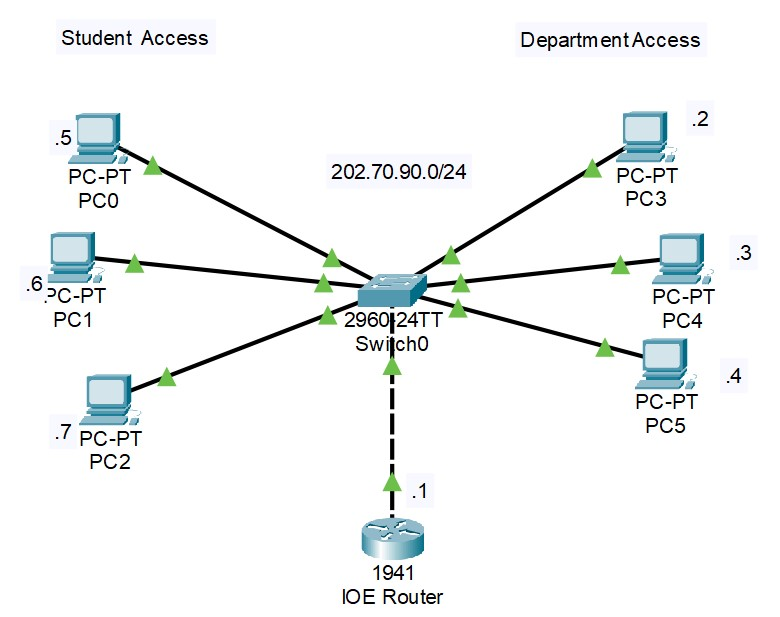
\includegraphics[scale=0.85,cframe=blue 0.5pt 3pt]{./IOEB.jpg}
            \caption{IOE network before subnetting}
        \end{figure}

        \begin{figure}[H]
            \centering
            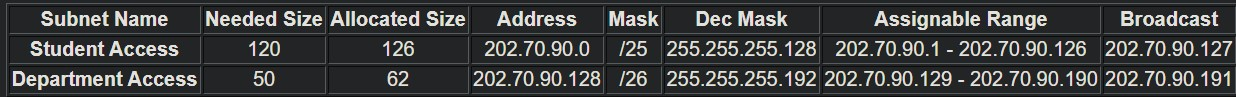
\includegraphics[scale=0.7,cframe=blue 0.5pt 3pt]{./SubTab.jpg}
            \caption{Details of IOE Subnets}
        \end{figure}


        \begin{figure}[H]
            \centering
            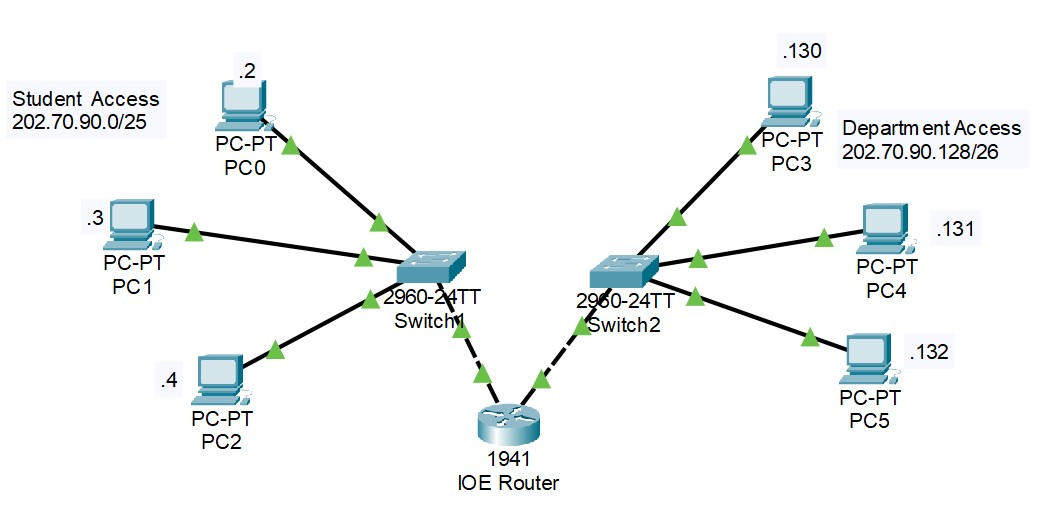
\includegraphics[scale=0.75,cframe=blue 0.5pt 3pt]{./IOEA.jpg}
            \caption{IOE network after subnetting}
        \end{figure}
    }
\end{A}
%%%%%%%%%%%%%%%%%%%%%%%%%%%%%%%%%%%%%%%%%%%%%%%%%%%%%%%%%%%%%%%%%

%%%%%%%%%%%%%%%%%%%%%5555555555555555555555555555

\begin{Q}
    {
        Suppose you have given the IP address of 102.5.4.0/23 for your company. There are five
        different departments having 200, 100, 40, 20 and 12 hosts. Two additional point-to-point
        links are there for interconnection between routers. Divide the given IP address for above
        requirements. List out the network address, broadcast address, usable IP address range and
        subnet mask of each subnet.
    }
\end{Q}


\begin{A}
    {

        As we know subnet can be created in Block size of $2^n$ number of host with ($2^n$ -2) usable host. So we have to choose the subnet equal to or greater than Block size after adding network and broadcast address.

        Starting with Department A we need 200 usable host so block size greater or qual to (200+2) is 256 with usable host 254.  Here \textbf{102.5.4.0 /24} will be network ID , \textbf{255.255.255.0 }will be subnet mask, \textbf{102.5.4.1 - 102.5.4.254} will  be available usable host range and \textbf{102.5.4.255} will be broadcast ID.

        Similarly for all other Department and 2 Interlink the required range is calculated and listed int he table below.
        There is unused Ip range from \textbf{102.5.5.248 - 102.5.255.255}.


        \begin{table}[H]
            \centering
            \setlength{\extrarowheight}{0pt}
            \addtolength{\extrarowheight}{\aboverulesep}
            \addtolength{\extrarowheight}{\belowrulesep}
            \setlength{\aboverulesep}{0pt}
            \setlength{\belowrulesep}{0pt}
            \begin{tabular}{ m{8em}| m{3em}| m{4em}| m{5em}| m{2em}| m{7em}| m{5em}| m{5em}| m{5em}|}
                \toprule
                \rowcolor[rgb]{0.416,0.702,0.961} \textbf{ Subnet Name }    & \textbf{ Needed Size } & \textbf{ Allocated Size } & \textbf{Network Address } & \textbf{ Mask } & \textbf{ Dec Mask } & \textbf{ Assignable Range } & \textbf{ Broadcast } \\
                \hline
                {\cellcolor[rgb]{0.129,0.816,0.557}}\textbf{ Department A } & 200                    & 254                       & 102.5.4.0                 & /24             & 255.255.255.0       & 102.5.4.1 -
                102.5.4.254                                                 & 102.5.4.255                                                                                                                                                                 \\
                \hline
                {\cellcolor[rgb]{0.129,0.816,0.557}}\textbf{ Department B } & 100                    & 126                       & 102.5.5.0                 & /25             & 255.255.255.128     & 102.5.5.1 -
                102.5.5.126                                                 & 102.5.5.127                                                                                                                                                                 \\
                \hline
                {\cellcolor[rgb]{0.129,0.816,0.557}}\textbf{ Department C } & 40                     & 62                        & 102.5.5.128               & /26             & 255.255.255.192     & 102.5.5.129 -
                102.5.5.190                                                 & 102.5.5.191                                                                                                                                                                 \\
                \hline
                {\cellcolor[rgb]{0.129,0.816,0.557}}\textbf{ Department D } & 20                     & 30                        & 102.5.5.192               & /27             & 255.255.255.224     & 102.5.5.193 -
                102.5.5.222                                                 & 102.5.5.223                                                                                                                                                                 \\
                \hline
                {\cellcolor[rgb]{0.129,0.816,0.557}}\textbf{ Department E } & 12                     & 14                        & 102.5.5.224               & /28             & 255.255.255.240     & 102.5.5.225 -
                102.5.5.238                                                 & 102.5.5.239                                                                                                                                                                 \\
                \hline
                {\cellcolor[rgb]{0.129,0.816,0.557}}\textbf{ Interlink 0 }  & 2                      & 2                         & 102.5.5.240               & /30             & 255.255.255.252     & 102.5.5.241 -
                102.5.5.242                                                 & 102.5.5.243                                                                                                                                                                 \\
                \hline
                {\cellcolor[rgb]{0.129,0.816,0.557}}\textbf{ Interlink 1 }  & 2                      & 2                         & 102.5.5.244               & /30             & 255.255.255.252     & 102.5.5.245 -
                102.5.5.246                                                 & 102.5.5.247                                                                                                                                                                 \\
                \bottomrule
            \end{tabular}
            \caption{Network address, broadcast address, usable IP address range and
                subnet mask}
        \end{table}
    }
\end{A}
%%%%%%%%%%%%%%%%%%%%%%%%%%%%%%%%%%%%%%%%%%%%%%%%%%%%%%%%%%%%%%%%%


%%%%%%%%%%%%%%%%%%%%%%%%%%%%666666666666666666666666666666
\begin{Q}
    {
        What is the count to infinity problem in distance vector routing? How can it be addressed?
        Explain with example.
    }
\end{Q}
\begin{A}
    {
        Distance Vector Routing is one of the dynamic routing algorithm in which Router maintain its routing table and informs its neighbors about  the distance to other node in the network. This routing technique has Count to infinity problem.

        When  an interface is down or  when two routers send updates at the same time, other routers unknowingly given information that they know how to reach a disconnected node. This false information will propagate to all routers and leading to infinity Loop problem of count to infinity. the following example will further clear the concepts.

        \begin{figure}[H]
            \centering
            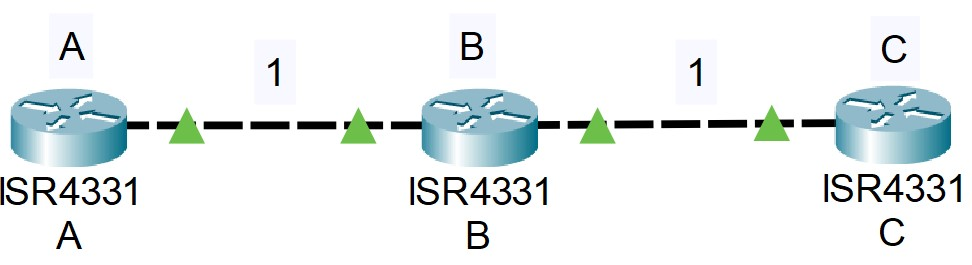
\includegraphics[scale=0.75,cframe=blue 0.5pt 3pt]{./CTI1.jpg}
            \caption{ Router A, B and C before breakage }
        \end{figure}

        In the above configuration Router B will know that it can reach to C at cost 1 , and A will know it can reach to C via B at the cost of 1.


        \begin{figure}[H]
            \centering
            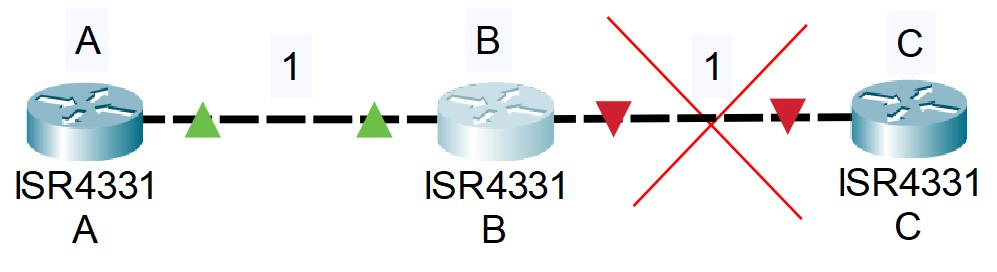
\includegraphics[scale=0.75,cframe=blue 0.5pt 3pt]{./CTI2.jpg}
            \caption{ Router A, B and C after breakage }
        \end{figure}

        What if the link between B and C disconnected , and B knows that it can no longer reach C and updates its Routing table . There is possibility that Router B receives update from Router A informing that it can reach C at cost of 2 , before B can broadcast its updated Routing table to its neighbors. In that case B will update its Routing table that it can reach C at cost of 3 via A. Similarly router A will update its routing table that it can reach C via B at cost of 4. This process for large no. of times or cost reaches very large number (infinity).

        There are several technique to prevent Count to infinity Problem. Two of them are explained below.

        \begin{itemize}
            \item \textbf{Route Poisoning:}

                  In Route poisoning whenever router detects bad route or router failure then that particular router inform its neighbors that cost to that router is higher than threshold and that router informs its other neighbors and remove that faulty route or router from its table.

                  For example when Router C is down it advertise the cost to C vis B is 16 which is above the threshold 15 , so Router A will remove information about router C from its routing Table.

            \item \textbf{Split horizon:}


                  Split horizons states that if a neighboring router sends a route to a router , the receiving router will not propagate this route back to the advertising router on the same interface.

                  In our example Router B won't inform updated router to Router A and prevent the further confusion and chance to count to infinity problem.


        \end{itemize}
    }
\end{A}
%%%%%%%%%%%%%%%%%%%%%%%%%%%%%%%%%%%%%%%%%%%%%%%%%%%%%%%%%%%%%%%%%

%%%%%%%%%%%%%%%%%%%%%%%%%%%%%%%777777777777777777777777777777777
\begin{Q}
    {
        What is unicast, multicast and broadcast? How does multicast differ from multiple unicast?
        Why do routers not forward broadcast packets? Explain.
    }
\end{Q}
\begin{A}
    {
        \textbf{Unicast} is common form of data transfer in which single sender send packets to a particular recipients. In simple terms it is one to one transmission.


        \textbf{Multicast} data transfer involves one sender and multiple recipients. In simple terms it is  one to many transmission.

        \textbf{Broadcast} data transfer involves one sender and all other host as receiver . it is one to all transmission.


        In multicast transmission there is multicast group identified by multicast address. here router duplicate the data packets direct to the destination host. However in multiple unicast sender direct the individual data packets to individual receiver all by itself increasing network traffic and wasting resources.


        Forwarding broadcast packets will be waste of resources and increase traffic congestion in the whole network as a single host is capable to populate the whole WAN(Internet) with garbage data.
    }
\end{A}
%%%%%%%%%%%%%%%%%%%%%%%%%%%%%%%%%%%%%%%%%%%%%%%%%%%%%%%%%%%%%%%%%

%%%%%%%%%%%%%%%%%%%%%%%%%%%%%%%8888888888888888888888888888888888888

\begin{Q}
    {
        Differentiate:
    }
\end{Q}

\begin{itemize}
    \item {\Large \textbf{ Distance vector vs. link state routing}}
          \begin{DT}{Distance vector}{Link state routing}
              Defination        & Each router computes distance between itself and~ its immediate neighbors. & Each router shares knowledge of its neighbors with every other router in the network.  \\
              Algorithm         & Bellman ford                                                               & Dijsktra                                                                               \\
              Best Route        & Least number of hops                                                       & Least cost                                                                             \\
              Updates frequency & Periodic updates                                                           & Triggered updates                                                                      \\
              Converge Time~    & Slower~                                                                    & Faster                                                                                 \\
              Problems          & Count to infinity~                                                         & Problems –~                                                                            \\
          \end{DT}



    \item {\Large \textbf{ IGP vs. EGP}}

          \begin{DT}{IGP}{EGP}
              Full form           & Interior Gateway Protocol (IGP) & Exterior Gateway Protocol (EGP)       \\
              Working area        & Within an~Autonomous System.    & Between different~Autonomous Systems  \\
              Colmplexity         & Simple                          & Complex                               \\
              Available Protocols & RIP, OSPF, ISIS, EIGRP          & RIP, OSPF, ISIS, EIGRP                \\
          \end{DT}

    \item {\Large \textbf{ SNAT vs. DNAT}}

          \begin{DT}{SNAT}{DNAT}
              Fullform            & Source Network Address Translation                                              & Destination Network Address Translation.                               \\
              Address Change      & Changes the source address of packets                                           & Changes the destination address of packets~                            \\
              Order of opreration & After the routing decision is made.                                             & Before the routing decision is made.                                   \\
              Working             & Convert the private IP address assigned by the router to the public IP address. & Forward the data coming in a public ip address to a private network.   \\
          \end{DT}

    \item {\Large \textbf{ ARP vs. RARP}}

          \begin{DT}{ARP}{RARP}
              Fullform        & Address Resolution Protocol.                                     & Address Resolution Protocol.                                       \\
              Address fetched & Receiver’s MAC address                                           & IP address is fetched.                                             \\
              Mapping         & ARP maps 32-bit logical (IP) address to 48-bit physical address. & RARP maps 48-bit physical address to 32-bit logical (IP) address.  \\
              Use             & Still in use                                                     & Replaced by DHCP                                                   \\
              Table upadate   & Uses ARP reply~                                                  & RARP reply for configuration of IP addresses .                     \\
          \end{DT}

\end{itemize}

%%%%%%%%%%%%%%%%%%%%%%%%%%%%%%%%%%%%%%%%%%%%%%%%%%%%%%%%%%%%%%%%%

%%%%%%%%%%%%%%%%%%%%%%%%%%%%%9999999999999999999999999999
\begin{Q}
    {
        Discuss briefly on:
    }
\end{Q}
\begin{A}
    {
        \begin{itemize}
            \item {\Large \textbf{ RIP:}}

                  Routing Information Protocol uses distance vector algorithm to maintain the routing tables.The cost metric is the number of hops to reach the destination. The number of hops available in a network would be the cost. The hop count is the number of networks required to reach the destination.In RIP, infinity is defined as 16, this will prevent count to infinity problem. The maximum number of hops that RIP can contain is 15 hops, i.e., it should not have more than 15 hops as 16 is infinity.Some advantages of RIP are easy to configure, less comlexity and less CPU utilization.



            \item {\Large \textbf{ OSPF:}}

                  Open Shortest Path First (OSPF) is an Interior Gateway Protocol (IGP) used to find the shortest path between source and destination.It uses Dijkstra's shortest path algorithm. After shortest path is found it is broadcasted to all routers.


            \item {\Large \textbf{ BGP:}}

                  Border Gateway Protocol (BGP) is one of the types of Protocol of Exterior gateway protocol (EGP) where the routers exchange network reachability information with their nearest neighbors.The neighbors then decide the shortest route to particular destination and update its table and then broadcast to its neighbors.To avoid
                  the count to infinity and looping problems the router sends routing information to another router with its own AS number included so that whenever it can check for routing loops by verifying if its AS number is present or not.


            \item {\Large \textbf{ ICMP:}}

                  Internet Control Message Protocol(ICMP) is used to transmit error messages.For example, if a packet of data is too large for a router, the router will drop the packet and send an ICMP message back to the original source for the data. Ping and Trace route are commonly used ICMP protocols.

        \end{itemize}
    }
\end{A}
%%%%%%%%%%%%%%%%%%%%%%%%%%%%%%%%%%%%%%%%%%%%%%%%%%%%%%%%%%%%%%%%%


\end{document}